\documentclass[a4paper,11pt]{ctexart}

\usepackage[top=1.8cm,bottom=1.8cm,left=2.1cm,right=2.1cm]{geometry}
\usepackage{amsmath,amssymb}
\usepackage{enumitem}
\usepackage{fancyhdr}
\usepackage{lastpage}
\usepackage{array}
\usepackage{graphicx}

\pagestyle{fancy}
\fancyhf{}
\renewcommand{\headrulewidth}{0pt}
\fancyfoot[C]{\small 第~\thepage~页\quad 共~\pageref{LastPage}~页}

\linespread{1.28}
\setlength{\parindent}{0pt}

\newcommand{\blank}[1][2.6cm]{\underline{\hspace{#1}}}

\begin{document}

\begin{center}
  {\Large\bfseries 华中科技大学 2024～2025 学年第一学期}\\[0.35em]
  {\Large\bfseries “微积分（B）”期中考试试卷（A 卷）}\\[0.6em]
  {\normalsize
    考试方式：\underline{\;\;闭卷\;\;}\quad
    考试日期：\underline{\;\;2024-11-16\;\;}\quad
    考试时间：8:30--11:00\quad
    考试时长：\underline{\;\;150\;\;} 分钟\\[0.35em]
    专业班级：\blank[3.0cm]\quad
    学号：\blank[3.0cm]\quad
    姓名：\blank[2.8cm]
  }
\end{center}

\begin{center}
  \renewcommand{\arraystretch}{1.35}
  \begin{tabular}{|c|*{4}{wc{1.75cm}|}}
    \hline
    题号 & 一 & 二 & 三 & 总分 \\
    \hline
    分数 & & & & \\
    \hline
  \end{tabular}
\end{center}

\vspace{0.8em}

\textbf{一、基本计算题（每小题 6 分，共 60 分）}

\begin{enumerate}[label=\arabic*., leftmargin=2em, itemsep=1.05em, topsep=0.5em]
  \item 设 $x_n = \dfrac{1}{n+1} + \dfrac{1}{n+\sqrt[3]{2}} + \cdots + \dfrac{1}{n+\sqrt[3]{n}}$，求 $\lim\limits_{n\to\infty} x_n$.

  \item 求极限 $l = \lim\limits_{x\to 0}\dfrac{e^x - e^{x\cos x}}{x\ln(1+x^2)}$.

  \item 当 $x\to 0$ 时，求无穷小量 $u = \left(\dfrac{2+\cos x}{3}\right)^{x^2} - 1$ 的主部和阶数.

  \item 求极限 $l = \lim\limits_{x\to 0}\dfrac{\sqrt{1-x^2}-\cos 3x}{e^x-1-x}$.

  \item 设函数 $f(x) = \dfrac{\sqrt{1+\sin x+\sin^2 x}-(\alpha+\beta\sin x)}{\sin^2 x}$，且点 $x=0$ 是 $f(x)$ 的可去间断点，试求常数 $\alpha,\beta$ 的值.

  \item 设 $y = \sqrt[3]{\dfrac{x(x^2+1)}{(x^2-1)^2}}$，求导数 $y'$.

  \item 设 $y = f(\sin^2 x)$，求 $y'$ 及 $y''$.

  \item 设 $f(x) = \begin{cases} (1+x^2)^{\frac{1}{\sin x}}, & x\neq 0, \\ 1, & x=0, \end{cases}$ 求 $f'(x)$.

  \item 设函数 $y=y(x)$ 是由方程 $\cos(xy)+\ln y - x - 1 = 0$ 确定的可微函数，求 $\left.dy\right|_{x=0}$.

  \item 设 $f(x) = x^2\ln(1+x)$，求 $f^{(6)}(0)$.
\end{enumerate}

\vspace{1.0em}
\textbf{二、综合题（每小题 6 分，共 30 分）}

\begin{enumerate}[label=\arabic*., start=11, leftmargin=2em, itemsep=1.05em, topsep=0.5em]
  \item 讨论函数 $f(x) = \lim\limits_{n\to\infty}\dfrac{x^2 e^{n(x-1)}+ax+b}{e^{n(x-1)}+1}$ 的连续性，其中 $a,b$ 为常数.

  \item 设函数 $y=f(x)$ 由参数方程 $\begin{cases} x=\arctan\sqrt{t}, \\ y=y(t) \end{cases}\ (t>0)$ 确定，其中 $y=y(t)$ 由方程 $e^y+e^t=2e$ 确定，求曲线 $y=f(x)$ 在点 $\left(\dfrac{\pi}{4},\, f\left(\dfrac{\pi}{4}\right)\right)$ 处的切线方程.

  \item 设数列 $\{x_n\}$ 满足 $x_1=1,\ x_n=x_{n-1}+\dfrac{1}{n^2}\ (n\ge 2)$，研究极限 $\lim\limits_{n\to\infty} x_n$ 的存在性.

  \item 在距火箭发射塔 $4000$ 米处安装一台摄像机，为使摄像机的镜头始终对准火箭，摄像机的仰角 $\theta$ 应随着火箭的上升不断增加（如图所示）. 假设火箭发射后垂直上升到距离地面 $3000$ 米处，其速度为 $600\text{ 米/s}$，试求在此时刻摄像机仰角 $\theta$ 的变化率.

  \begin{center}
    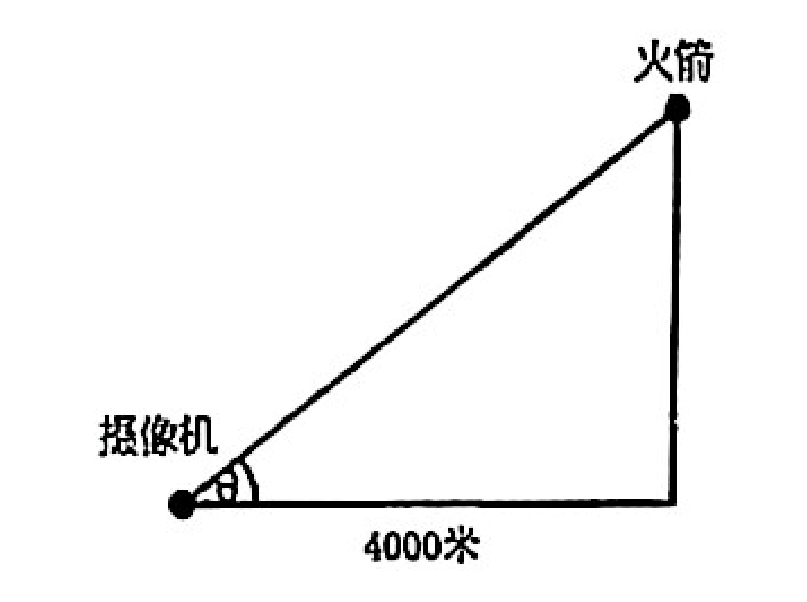
\includegraphics[width=0.28\textwidth]{assets_文字版/doc27_q14.png}
  \end{center}

  \item 设可微函数 $y=f(x)$ 由方程 $x^3+y^3+xy-1=0$ 确定，求 $\lim\limits_{x\to 0}\dfrac{f(\cos x-1)-1}{\ln(1+x^2)}$.
\end{enumerate}

\vspace{1.0em}
\textbf{三、证明题（每小题 5 分，共 10 分）}

\begin{enumerate}[label=\arabic*., start=16, leftmargin=2em, itemsep=1.05em, topsep=0.5em]
  \item 设正整数 $n>1$，证明：$x^{2n}+a_1x^{2n-1}+a_2x^{2n-2}+\cdots+a_{2n-1}x-1=0$ 至少有两个实根.

  \item 设函数 $f(x)$ 在 $[0,1]$ 上连续，在 $(0,1)$ 内可导，并且 $f(0)=f(1)=0,\ f\left(\dfrac{1}{2}\right)=1$，证明存在 $\xi\in(0,1)$，使得 $f'(\xi)=1$.
\end{enumerate}

\end{document}
